\documentclass[smallextended]{svjour3}

%% Language and font encodings
\usepackage[english]{babel}
\usepackage[utf8x]{inputenc}
\usepackage[T1]{fontenc}

%% Sets page size and margins
\usepackage[a4paper,top=3cm,bottom=2cm,left=3cm,right=3cm,marginparwidth=1.75cm]{geometry}

%% Useful packages
\usepackage{amsmath}
\usepackage{graphicx}
\usepackage[colorinlistoftodos]{todonotes}
\usepackage[colorlinks=true, allcolors=blue]{hyperref}
\usepackage{subcaption}

\title{TER Report - Interior 3D detection in a cobotics context}

\author{BIZARD Astor  \\ \and \\
      Supervised by : Olivier Aycard  \and Jerôme Maisonnasse
}

\institute{
}

\date{June 2017}

\begin{document}
\maketitle

\begin{abstract}
We present an approach to compute 3D data in a real-time security context to evaluate distance between humans and robots. The implementation is oriented to be compatible with the ROS platform, and overcome drawbacks of low-quality depth cameras, such as important noise.
\keywords{3D Depth Sensor \and RGB-D Perception \and Collision Avoidance \and ROS \and Physical Human-Robot Interaction}
\end{abstract}

\section{Introduction}

The problem of collaboration between humans and industrial robots - also known as cobotics - induces security issues : how to ensure the security of the human, without limiting the possibilities of the collaboration ? We thus need to find a way to do this without preventing the humans to approach the robot. The work must therefore be done on limiting the robot moves to a secure zone, calculated knowing the position of the persons. This limit must be computed in reasonable time to ensure security.

\section{A static vision approach}

We need a way to perceive the 3D environment in which the robot moves. Using 3D depth sensors seems a pretty good way to get an estimation of a part of this environment.

\subsection{Where to place the sensors}

\subsubsection{On the robot itself}

In many situations where robots need to perceive their environment (using a perception-decision-action scheme), the sensors are intuitively placed on the robot, as a human got his eyes and ears on himself to perceive its own environment. But there are some robots that cannot handle sensors on their bodies : for example industrial arms that move in every direction cannot give a reliable perception (cf Fig. \ref{fig:robotic_arm}).

\subsubsection{Static sensors}

A different an more reliable way to get informations is to place static sensors. The advantage of this method is that we can use several sensors to cover a wider range in the room, and that without obstructing the robot's or human's movement. It however requires the presence of several sensors, as objects or persons could possibly hide the robot and compromise the availability of reliable information.


\begin{figure}
\centering
\includegraphics[width=0.5\textwidth]{robotic_arm.jpg}
\caption{\label{fig:robotic_arm}A typical application of cobotics with an industrial robotic arm.}
\end{figure}

\subsection{The ROS API}

One of the most used API in the world of robotics is the ROS platform. It works as a set of executables, named nodes, which communicate with messages published on topics. The advantage of this platform is that it provides a standardized API for communicating with autonomous robots. In our case, we present a solution with two nodes, added to the sensor node : the first one will be charged to analyze the data provided by the sensor, identifying moving objects and persons ; the second one will check - from the information given by the first node - that the human security is not compromised.

\section{Clusterisator node A CHANGER DE NOMAAAAAAAAAAAAAAAAAAAAAAAAAAAAAAAAAAAAAAAAAAAAAA}

\subsection{Sensor data}

\begin{figure}
\centering
\includegraphics[width=0.4\textwidth]{depth_space.png}
\caption{\label{fig:depth_space}Representation of the Depth space \cite{Ref1}.}
\end{figure}

We are using low-cost RGB-D cameras, with the OpenNI standard - we are working with the ASUS XTion PRO LIVE model. We are using the openni\_camera node of ROS \cite{Refopenni} to get data as a ROS message.

\subsubsection{Depth space}
A depth camera provides data in a implicit depth space (cf Fig. \ref{fig:depth_space}) : a distance is given for each pixel of the image. Posing d as the distance at the pixel (i,j), we get the point (i,j,d) in the depth space with the camera as the origin.

\subsection{Noise minimization}

The cameras we are using are cheap, but it indeed has drawbacks, such as important noise (cf Fig. \ref{fig:camera1}) : these cameras use infra-red projection to get the depth data - cheaper than laser but less effective. We get noise on these images (see black dots on Fig. \ref{fig:camera1}), often on smooth or glossy surfaces.

\begin{figure}
\centering
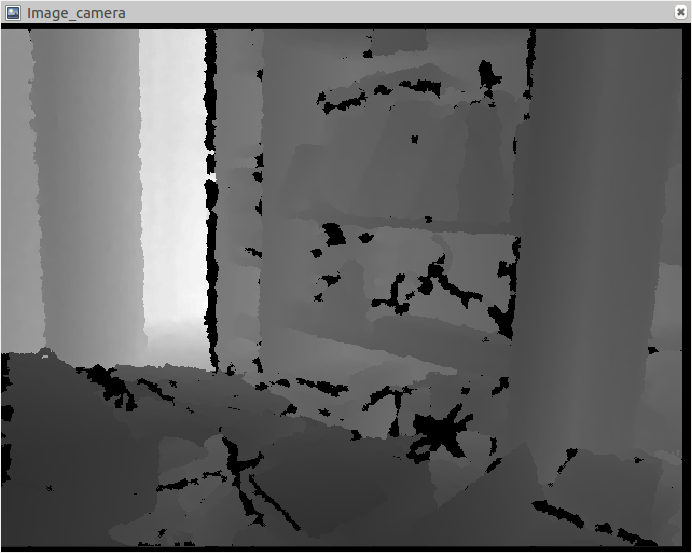
\includegraphics[width=0.5\linewidth]{camera_01.png}
\caption{\label{fig:camera1}The depth image, as received by the camera : dark points are near the camera, bright ones are far.}
\end{figure}

\begin{figure}
\centering
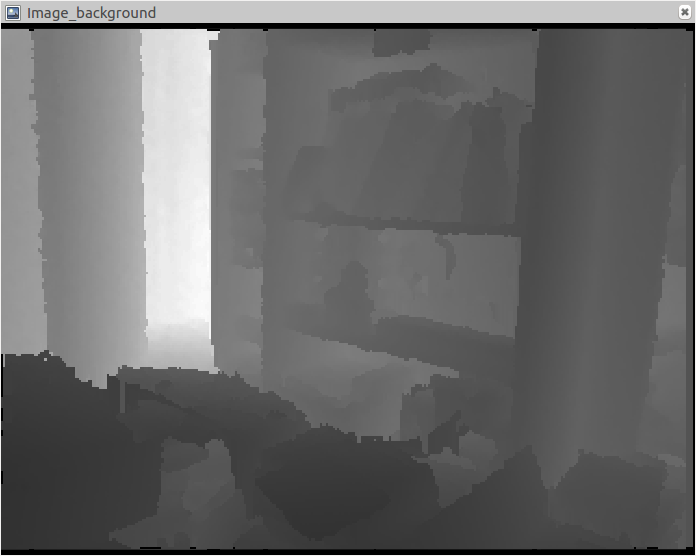
\includegraphics[width=0.5\linewidth]{background_01.png}
\caption{\label{fig:background1}The same depth image after noise treatment.}
\end{figure}

\subsection{Clustering}

\subsection{Identification}

\section{Securistator node A CHANGER DE NOMAAAAAAAAAAAAAAAAAAAAAAAAAAAAAAAAAAAAAAAAAAAAAAAAAAAAA}


\begin{figure}
\centering
\includegraphics[width=0.6\textwidth]{depth_cartesian_spaces.png}
\caption{\label{fig:spaces}Representation of Cartesian space (a) and Depth space (b) \cite{Ref1}.}
\end{figure}

\subsection{How to add Tables}

Use the table and tabular commands for basic tables --- see Table~\ref{tab:widgets}, for example. 

\begin{table}
\centering
\begin{tabular}{l|r}
Item & Quantity \\\hline
Widgets & 42 \\
Gadgets & 13
\end{tabular}
\caption{\label{tab:widgets}An example table.}
\end{table}

\subsection{How to write Mathematics}

\LaTeX{} is great at typesetting mathematics. Let $X_1, X_2, \ldots, X_n$ be a sequence of independent and identically distributed random variables with $\text{E}[X_i] = \mu$ and $\text{Var}[X_i] = \sigma^2 < \infty$, and let
\[S_n = \frac{X_1 + X_2 + \cdots + X_n}{n}
      = \frac{1}{n}\sum_{i}^{n} X_i\]
denote their mean. Then as $n$ approaches infinity, the random variables $\sqrt{n}(S_n - \mu)$ converge in distribution to a normal $\mathcal{N}(0, \sigma^2)$.


\subsection{How to create Sections and Subsections}

Use section and subsections to organize your document. Simply use the section and subsection buttons in the toolbar to create them, and we'll handle all the formatting and numbering automatically.

\subsection{How to add Lists}

You can make lists with automatic numbering \dots

\begin{enumerate}
\item Like this,
\item and like this.
\end{enumerate}
\dots or bullet points \dots
\begin{itemize}
\item Like this,
\item and like this.
\end{itemize}

\subsection{How to add Citations and a References List}

You can upload a \verb|.bib| file containing your BibTeX entries, created with JabRef; or import your \href{https://www.overleaf.com/blog/184}{Mendeley}, CiteULike or Zotero library as a \verb|.bib| file. You can then cite entries from it, like this: \cite{greenwade93}. Just remember to specify a bibliography style, as well as the filename of the \verb|.bib|.

You can find a \href{https://www.overleaf.com/help/97-how-to-include-a-bibliography-using-bibtex}{video tutorial here} to learn more about BibTeX.

We hope you find Overleaf useful, and please let us know if you have any feedback using the help menu above --- or use the contact form at \url{https://www.overleaf.com/contact}!

%\bibliographystyle{alpha}
%\bibliography{sample}
\begin{thebibliography}{}

\bibitem{Ref1}
F. Fabrizio and A. De Luca, Real-time computation of distance to dynamic obstacles with multiple depth sensors, IEEE Robotics and automation Letters (2016)

\bibitem{Refopenni}
http://wiki.ros.org/openni\_camera

\end{thebibliography}

\end{document}
